% !TEX root = ../main.tex

\chapter{顶层架构与模块}
这一章将详细阐述芯片的顶层架构设计,并对所涉及到的模块功能进行建模。
本章将分为三个部分,分别对架构设计、CIS数据通路中的模块设计、存储器的选择和设计进行深入的讨论。
整个设计过程是自顶向下的,因此完成这一章的顶层架构设计后,就可以在后续的章节展开对深度学习神经网络加速器和ResNet18网络固化到芯片上的讨论。


\section{架构设计}
架构的设计过程包括了需求分析、详细设计和建模。


\subsection{需求分析}
在进行架构设计和具体的模块设计之前,先对需求进行分析和总结。
这一小节将分析需要完成哪些设计和模型,来实现和验证在CIS芯片上的基于脉动阵列的ResNet18硬件加速运算。


\paragraph{基本设定}

%首先,我们先假设使用的CPU、总线、DRAM、SRAM都是理想状态。
在本课题中,首先需要设计CIS芯片的主体架构。
CIS芯片的主体架构包括了CPU、总线、ROM、SRAM、DRAM以及图像数据信号通路上的各个模块。
CPU和总线是芯片上必不可少的设备。
CPU能够执行程序和处理外设发出的中断。
总线是芯片上各个功能部件之间信息传输的干线。
常用的片上总线是AHB总线。AHB总线是有主机、从机和其他基础设施构成的。
基础设施中包含了仲裁器、数据的多路选择器、地址的多路选择器、译码器。
但本课题中的深度学习算法的运算将全部由专门的硬件加速部件来完成运算,因此下文将不再具体展开CPU和总线的类型和设计。
关于存储设备,本课题将讨论选用存储器的种类和不同种类存储器所需要的存储大小。
因为通常在一些小型的CIS中,芯片所需的内存很少,所以只需要选用SRAM就可以满足系统的需要。
在考虑到深度学习神经网络的模型的大小,同时也参考了一些业内的深度学习神经网络运算专用芯片,本课题中的设计将同时使用SRAM和DRAM。

% 内存大小的设计

\subsection{详细需求}
%讨论详细需求。
% 用例

% 需求分析
因此,我们可以分解需求,并得到以下列出的需求点:
\begin{enumerate}
    \item CIS的基础模块
    \item 图像处理模块
    \item 脉动阵列的设计
    \item ResNet18在脉动阵列上的实现
\end{enumerate}    

对于图像处理模块,需要设计一个配合脉动阵列工作的数据信号输入模块。
这个模块需要根据后文描述的脉动阵列运算的行为,将视频数据流中的数据按照脉动阵列所需的顺序放置到脉动阵列的输入缓冲中。
在脉动阵列中,需要设计每个处理单元的逻辑和工作行为。
在实现神经网络算法时,需要分解出所有使用到的运算符,并分析哪些可以通过脉动阵列的乘加运算矩阵加速。


\subsubsection{图像数据通路}
图像数据通路的需求是深度学习加速器的基础。
CIS芯片的作用,就是将图像传感器接收到的信号,转为数字信号后传输给后端。
芯片上图像数字信号所经过的所有模块连接起来就像是一条单向的通道。
一般的,我们称这些模块所组成的通道为图像数据通路。
图像数据通路一般由输入、数据处理和输出三个部分组成。
通常地,这三个部分也具有各自不同的时钟域。

%TODO 架构图展示
\begin{figure}[htbp]
    \centering
    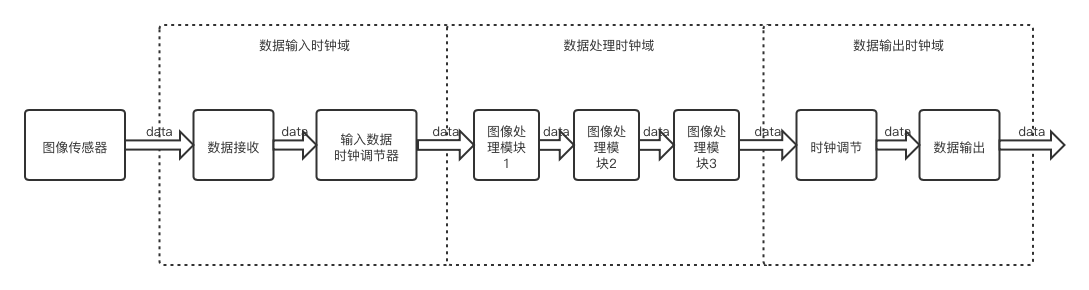
\includegraphics[width=15cm,height=5cm]{figures/datapath.png}
    \caption{图像信号处理的数据流图}
    \label{fig:datapath}
\end{figure}

%TODO 这里先描述以下datapath,包括DI、DP、DO三个时钟域。
如图\ref{fig:datapath}所示,图像处理部件的前后分别需要设置两个不同的时钟域用于输入和输出图像数据的信号。
因此,我们在设计CIS的数据通路中的深度学习运算模块时,也需要做相同的设计。
将输入模块的图像数据信号按一定的顺序排列好,按照脉动阵列的特性以一定的方式依次输入到阵列中。


在输入时钟域中,RX模块接收从CMOS传感器输出的数据。
由一个缓冲区暂存数据,经过时钟同步和一些预处理后向后面的数据处理时钟域输出数据。
在数据处理的时钟域中,深度学习运算模块将进行推理操作。
在输出时钟域中,FT(fix timing)模块将调整输出的时钟频率.TX模块负责以指定格式输出图像数据。  


\subsubsection{ResNet18中的基本运算}
选择ResNet18在此设计中实现的主要原因是ResNet18结构简单且图像识别正确率出众。
除了一开始的7x7卷积核,在实现运算的BasicBlock中的卷积运算全部采用的3x3的卷积核。
这样既可以把如何进行卷积运算的设计表达清楚,也可以避免过多地描述卷积神经网络算法本身。

% TODO 简述ResNet18的网络结构
ResNet18由4个主要的残差层组成。
整个网络的开头,由7x7的卷积核做卷积运算和3x3的最大池化。
卷积运算有64个输出的通道。设定的步长是2,填充的边框是3。
最大值池化的步长是2,填充的边框是1。
最后输出的图像尺寸是112x112

之后是四个包含两个BasicBlock来做运算的残差层。
每个BasicBlock中都有两个3x3的卷积运算。
它们的深度不同,分别是64、128、256和512。
ResNet可能使用两种不同的残差单元。一种是BasicBlock,用于ResNet18和ResNet34这种浅层网络。
另一种是Bottleneck,用于50层及以上的ResNet。

第一个残差层的卷积运算有64个输出通道。其输出的图像尺寸是56x56。
第二个残差层的卷积运算有128个输出通道。其中输出的图像尺寸是28x28。
第三个残差层的卷积运算有256个输出通道。其中输出的图像尺寸是14x14。
第四个残差层的卷积运算有512个输出通道。其中输出的图像尺寸是7x7。
最后,以平均池化、全连接和softmax结束整个resnet18网络。

% TODO 展开7x7卷积运算。
% TODO 

将特征图经过批归一化和Relu()激活函数。这两个运算不会改变特征图的维度。
% TODO 展开BN和Relu激活函数

之后用3x3的卷积核将特征图进行最大池化,步长为2,边框填充为3,得到56x56x64的特征图。
% TODO 展开3x3的maxpooling

后面就开始将数据依次输入4个残差层。
% TODO 展开残差层的计算
残差层包含了两个BasicBlock。因此它的运算可以参考上面的代码段中BasicBlock类的内容。
首先,输入从上一层得到的56x56x64的特征图。
将这个特征图用3x3x64的卷积核做卷积运算。使用的步长为1,填充的边框为1,得到56x56x64的特征图输出。
假设输入的特征图大小为m,卷积核大小为x,步长为s,边框填充层数为p,那么输出的特征图大小 $m^{'}$ 由公式(2-1)计算得到:
\begin{equation}
m^{'} = \frac{( m + 2 \times p - x )}{s} + 1 
\end{equation}  


下面是ResNet18所涉及到的所有运算:
\begin{enumerate}
    \item 2D卷积运算
    \item 批归一化
    \item 最大值池化
    \item Relu()激活函数
    \item 平均值池化
    \item 全连接
\end{enumerate}


\subsection{详细设计}
CIS的顶层架构设计是由CPU、高速总线、存储以及数据通路上的各个外设组成。
在后续的讨论中,将会把CPU、高速总线、存储器等基础组件做为设计内容中的一些设定。
本文将假设输入到深度学习运算模块的数据流,是一种理想的图像数据。
对于CIS上深度学习运算模块的设计,我们首先可以参考ISP芯片的设计逻辑。
因为我们可以将深度学习运算模块也视作一种图像处理的模块。

从图\ref{fig:top_arch}中可以看到,这是图像传感器与ISP以及其他功能部件连接在一条高速数据总线的结构。
总体架构可以分为几个部分:数据通路部分、系统控制部分和高速数据总线。
数据通路部分包含了IDA(Input Data Adapter)、深度学习神经网络加速模块、TX输出模块。
系统控制部分包含了CPU、DMA、Memory、SPI Flash以及其他外设模块(比如$I^2C$和UART等接口模块)。
%TODO 架构图展示
\begin{figure}[htbp]
    \centering
    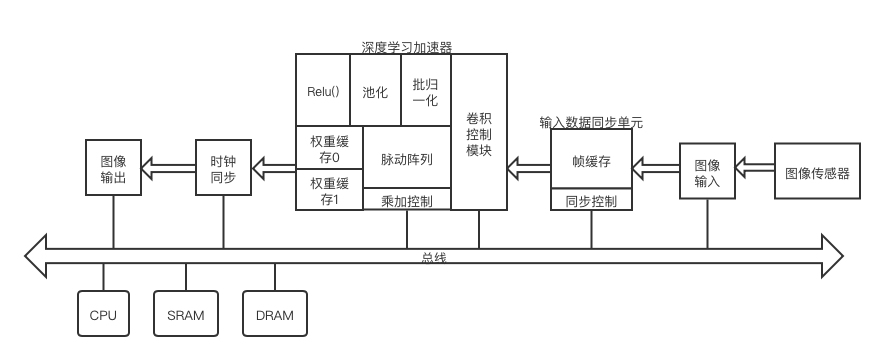
\includegraphics[width=15cm,height=6cm]{figures/top_arch.png}
    \caption{总体架构图}
    \label{fig:top_arch}
\end{figure}
%TODO 各个模块的简述
这里的视频数据格式设定为RGB888。



\subsection{详细设计}

\section{CIS数据通路}
%TODO 展示Stream datapath的传输方式 sof eof href
%TODO DL accelerator在数据通路中的作用
%TODO Fix Timing模块做数据同步,最后输出结果
图像数据通路的设计是本课题的核心部分。
本章将分别阐明数据流的输入,数据的运算,数据流的输出三个部分的所有模块设计原理。
其中,各小节会着重描述数据流的组件间逻辑关系,以及各个模块控制流的状态机和执行逻辑。
图像数据通路的整体设计如图所示\ref{fig:image_datapath},在整个图像数据通路中有三个不同的时钟域。
\begin{figure}[htbp]
    \centering
    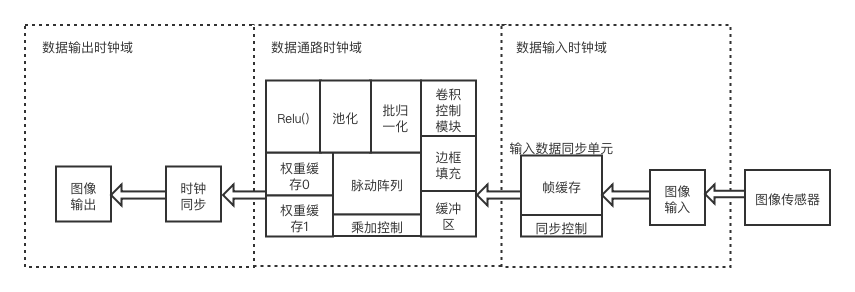
\includegraphics[width=15cm,height=6cm]{figures/image_datapath.png}
    \caption{图像数据通路架构图}
    \label{fig:image_datapath}
\end{figure}
区分这三个时钟域的目的是支持3个不同的时钟频率。
它们分别是图像传感器的输入数据信号的时钟、深度学习加速器的运行时钟和特征图的输出数据信号的时钟。
在这个数据通路中,最重要的模块就是深度学习运算加速器模块。


\subsection{数据流的输入}
% TODO 
%   数据流的输入将由IDA(Input Data Adapter)模块处理。这个模块的主要作用是将Sensor输出的数据放到一个缓存区。
%   并将视频数据流的plck同步到数据流的时钟域。

这里假设从图像传感器输出的图像数据为224x224像素尺寸的图像。
视频数据流的输入需要参考流式设备的特性,合理的缓存大小和同步的时机是关键点。
对于卷积运算,缓存的行数大小应该大于等于卷积核的行数和列数之间的较大值。
例如,卷积核的尺寸为3x3时,缓存至少要保存3行数据。
如果,每帧图像的尺寸为224x224个像素点。
由RGB三个通道组成的每一帧都拆分成三个224x224x8比特流。
那么需要给一个通道的一帧数据缓存的大小需要大于等于672个字节。

\begin{figure}[htbp]
    \centering
    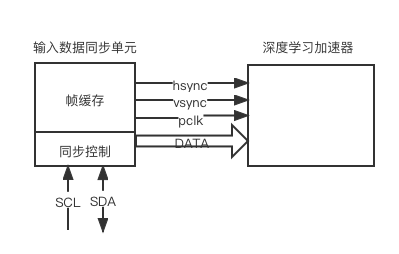
\includegraphics[width=12cm,height=8cm]{figures/input_data_adapter.png}
    \caption{输入数据同步单元架构图}
    \label{fig:input_data_adapter}
\end{figure}

如图\ref{fig:input_data_adapter}是数据输入同步单元与深度学习加速器之间的连线设计。
hsync用于行同步信号。
vsync用于帧同步信号。
pclk是像素时钟信号。
data是并行的图像数据,这里设定为8bit带宽。
SCL和SDA是用来读写模块寄存器的I2C接口的时钟信号和数据信号。


\subsection{数据流中的运算}
% TODO
% 在数据流中实时运算图像识别的算法
深度学习运算加速器是专用于进行深度学习运算的硬件加速模块。
它的作用是在数据通路中实时地进行图像识别的运算。
此设计选择了ResNet18作为实现的网络算法。
运算的模块将通过帧同步信号和行同步信号等机制来处理缓存的数据。
在实际应用时,将用于图像识别的人工智能处理器在物理位置上比较靠近图像来源(CMOS传感器),这样就避免了图像数据需要SRAM/DRAM的存储。
同时,还可以利用图像数据流的流水线特性,设计减小输入缓冲的图像输入模块。
依靠图像数据信号中的行同步信号和帧同步信号,来同步向数据通道后方的脉动阵列输送数据,那么就不需要缓冲多帧或者一个完整帧的数据。
另外,由于一般的CNN算法是共享权重的。这样权重的数量就不大,可以完整存放在片上SRAM中,从而使得读取权重的操作也能避免访问DRAM。
在设计权重缓冲区时,我们采用了多路缓冲的思想。将划分多个bank缓冲区,来分别缓冲不同卷积层的权重。
这样的话,权重缓冲区可以在脉动阵列工作时,加载后一层的权重到缓冲区中。
在需要进行下一层的运算时,脉动阵列就可以直接从SRAM的缓冲区中读取权重,而不是DRAM。
这样处理后,整个系统将大幅降低功耗。
% 单独画图解释一下权重缓冲区
% 单独画图解释一下行同步信号控制数据输入

整个深度学习加速器模块有2个缓存分别用于存储权重、输入数据。
核心的运算模块是由最小运算单元组成的脉动阵列。
普通的运算阵列受限于其规模。它的规模越大,需要的传输布线长度约长,传输时间越久,因此频率也无法做到很高。
这样的话,它的运算性能就会受到规模大小的限制。



\subsubsection{ResNet18的控制逻辑}
在深度学习加速器中的深度网络控制模块是一个固化了ResNet18残差网络\cite{resnet2015}的逻辑单元。
这个子模块将控制整个深度学习加速器的运算逻辑。
它控制的是ResNet18网络中每一层所做的工作。
深度学习控制模块将通过下面的状态机来控制这个控制流:
\begin{enumerate}
    \item 准备状态:当图像帧或者特征图已经完整地写入到缓冲区后,控制模块进入准备状态。在准备状态中,控制器将控制指定的运算模块做好运算前的,载入特征图数据到脉动阵列的输入通道中或是权重数据。
    \item 运行状态:在特征图和权重都载入到相应的缓冲区后,控制模块将驱动脉动阵列或者是相应的算数逻辑运算单元开始工作。这个运算模块工作的状态称为运行状态。
\end{enumerate}  
%TODO 这里增加一个状态机的图 在草稿纸上。
如图\ref{fig:resnet18_arch}是ResNet18的网络结构图。
\begin{figure}[htbp]
    \centering
    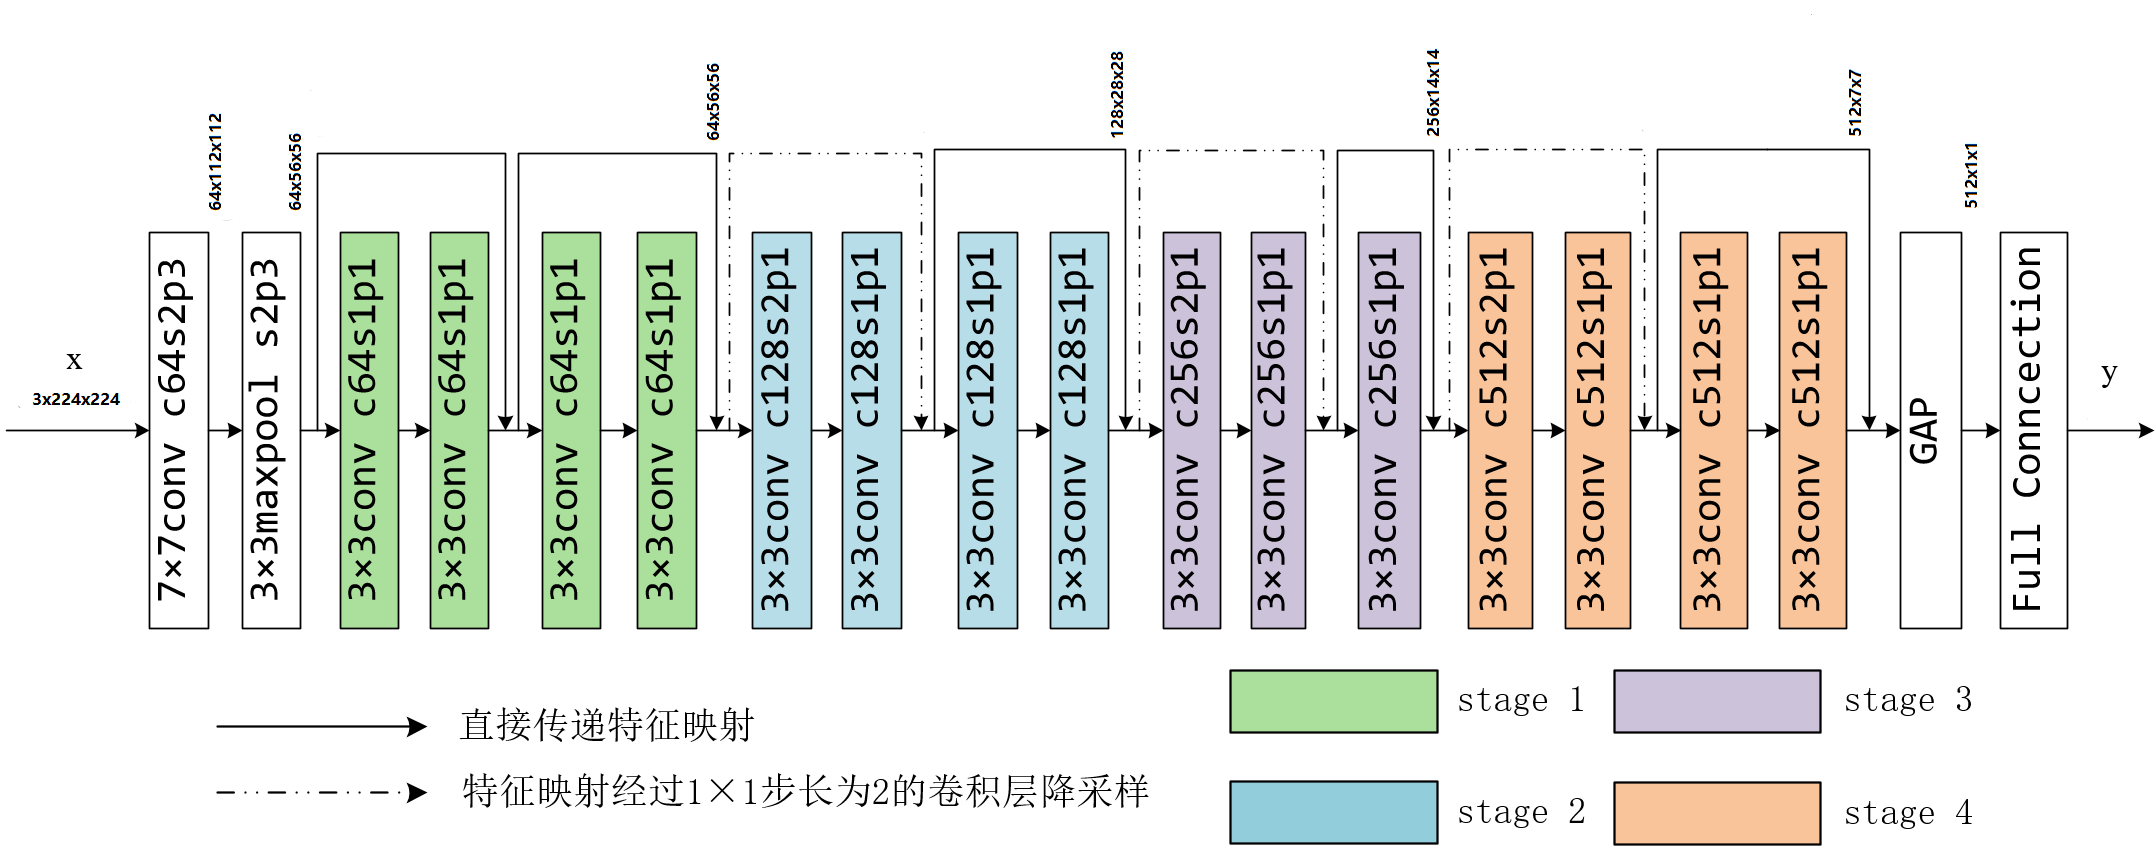
\includegraphics[width=12cm,height=5cm]{figures/resnet18_arch.png}
    \caption{ResNet18网络结构图}
    \label{fig:resnet18_arch}
\end{figure}

如表\ref{tab:output_shape_and_param}记录了ResNet18的所有隐含层、输出特征图的尺寸和这一层的参数个数。

%TODO 这里通过表格展示ResNet18的数据流。
\begin{table}[!hpt]
    \bicaption[ResNet18的输出数据尺寸和参数]{ResNet18的输出数据尺寸和参数}{Output shape and param of ResNet18}
    \label{tab:output_shape_and_param}
    \centering
    \begin{tabular}{@{}llllllllllll@{}} \toprule
        Num & Layer         & Output Shape      & Param   &  Num & Layer        & Output Shape      & Param         \\ 
        1  & Conv2d         & [112, 112, 64]    & 9408    &  41 & BatchNorm2d   & [14, 14, 256]     & 512           \\
        2  & BatchNorm2d    & [112, 112, 64]    & 128     &  42 & ReLU          & [14, 14, 256]     & 0             \\
        3  & ReLU           & [112, 112, 64]    & 0       &  43 & BasicBlock    & [14, 14, 256]     & 0             \\
        4  & MaxPool2d      & [112, 112, 64]    & 0       &  44 & Conv2d        & [14, 14, 256]     & 589824        \\
        5  & Conv2d         & [56, 56, 64]      & 36864   &  45 & BatchNorm2d   & [14, 14, 256]     & 512           \\
        6  & BatchNorm2d    & [56, 56, 64]      & 128     &  46 & ReLU          & [14, 14, 256]     & 0             \\
        7  & ReLU           & [56, 56, 64]      & 0       &  47 & Conv2d          & [14, 14, 256]     & 589824      \\
        8  & Conv2d         & [56, 56, 64]      & 36864   &  48 & BatchNorm2d     & [14, 14, 256]     & 512         \\
        9  & BatchNorm2d    & [56, 56, 64]      & 128     &  49 & ReLU            & [14, 14, 256]     & 0           \\
        10 & ReLU           & [56, 56, 64]      & 0       &  50 & BasicBlock      & [14, 14, 256]     & 0           \\
        11 & BasicBlock     & [56, 56, 64]      & 0       &  51 & Conv2d          & [7, 7, 512]       & 1179648     \\
        12 & Conv2d         & [56, 56, 64]      & 36864   &  52 & BatchNorm2d     & [7, 7, 512]       & 1024        \\
        13 & BatchNorm2d    & [56, 56, 64]      & 128     &  53 & ReLU            & [7, 7, 512]       & 0           \\
        14 & ReLU           & [56, 56, 64]      & 0       &  54 & Conv2d          & [7, 7, 512]       & 2359296     \\
        15 & Conv2d         & [56, 56, 64]      & 36864   &  55 & BatchNorm2d     & [7, 7, 512]       & 1024        \\
        16 & BatchNorm2d    & [56, 56, 64]      & 128     &  56 & Conv2d          & [7, 7, 512]       & 131072      \\
        17 & ReLU           & [56, 56, 64]      & 0       &  57 & BatchNorm2d     & [7, 7, 512]       & 1024        \\
        18 & BasicBlock     & [56, 56, 64]      & 0       &  58 & ReLU            & [7, 7, 512]       & 0           \\
        19 & Conv2d         & [28, 28, 128]     & 73728   &  59 & BasicBlock      & [7, 7, 512]       & 0           \\    
        20 & BatchNorm2d    & [28, 28, 128]     & 256     &  60 & Conv2d          & [7, 7, 512]       & 2359296     \\    
        21 & ReLU           & [28, 28, 128]     & 0       &  61 & BatchNorm2d     & [7, 7, 512]       & 1024        \\         
        22 & Conv2d         & [28, 28, 128]     & 147456  &  62 & ReLU            & [7, 7, 512]       & 0           \\      
        23 & BatchNorm2d    & [28, 28, 128]     & 256     &  63 & Conv2d          & [7, 7, 512]       & 2359296     \\    
        24 & Conv2d         & [28, 28, 128]     & 8192    &  64 & BatchNorm2d     & [7, 7, 512]       & 1024        \\
        25 & BatchNorm2d    & [28, 28, 128]     & 256     &  65 & ReLU            & [7, 7, 512]       & 0           \\
        26 & ReLU           & [28, 28, 128]     & 0       &  66 & BasicBlock      & [7, 7, 512]       & 0           \\
        27 & BasicBlock     & [28, 28, 128]     & 0       &  67 & AdaptiveAvgPool & [1, 1, 512]       & 0           \\
        28 & Conv2d         & [28, 28, 128]     & 147456  &  68 & Linear          & [2]               & 1026        \\
        29 & BatchNorm2d    & [28, 28, 128]     & 256     &     &                 &                   &             \\
        30 & ReLU           & [28, 28, 128]     & 0       &     &                 &                   &             \\  
        31 & Conv2d         & [28, 28, 128]     & 147456  &     &                 &                   &             \\  
        32 & BatchNorm2d    & [28, 28, 128]     & 256     &     &                 &                   &             \\  
        33 & ReLU           & [28, 28, 128]     & 0       &     &                 &                   &             \\  
        34 & BasicBlock     & [28, 28, 128]     & 0       &     &                 &                   &             \\  
        35 & Conv2d         & [14, 14, 256]     & 294912  &     &                 &                   &             \\  
        36 & BatchNorm2d    & [14, 14, 256]     & 512     &     &                 &                   &             \\  
        37 & ReLU           & [14, 14, 256]     & 0       &     &                 &                   &             \\  
        38 & Conv2d         & [14, 14, 256]     & 589824  &     &                 &                   &             \\  
        39 & BatchNorm2d    & [14, 14, 256]     & 512     &     &                 &                   &             \\  
        40 & Conv2d         & [14, 14, 256]     & 32768   &     &                 &                   &             \\  

    \end{tabular}
\end{table}

\subsubsection{脉动数据和统一数据缓冲区}
在设计脉动阵列的逻辑时,它与普通的深度学习运算单元组成的网络的区别是需要把输入脉动阵列的数据按照一定的顺序排列好。
并且按照一定的节奏输送到脉动阵列中。
如图\ref{fig:systolic_data}所示,是一个对一个5x5大小输入的特征图用2个3x3的卷积核做卷积运算的示意图,用来说明怎样对输入脉动阵列的数据进行排序和分组的。
如图\ref{}是脉动阵列的输入数据和权重。
图中,左侧的由两位数字组成的标号表示了它在5x5的矩阵中的位置。
右侧的两列分别是W0和W1的两个卷积核的数据平铺展开得到的。
0到8的编号表示了它们在两个卷积核中的位置。

%DONE 这里插入一个对一个5x5的输入用3x3的卷积核做卷积运算的示意图
\begin{figure}[htbp]
    \centering
    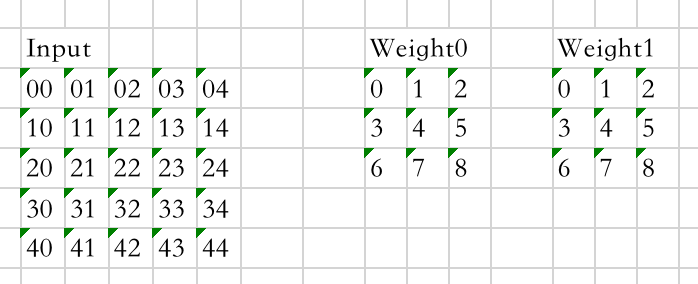
\includegraphics[width=15cm]{figures/my_systolic_input.png}
    \caption{输入和权重示意图}
    \label{fig:systolic_data}
\end{figure}


\begin{figure}[htbp]
    \centering
    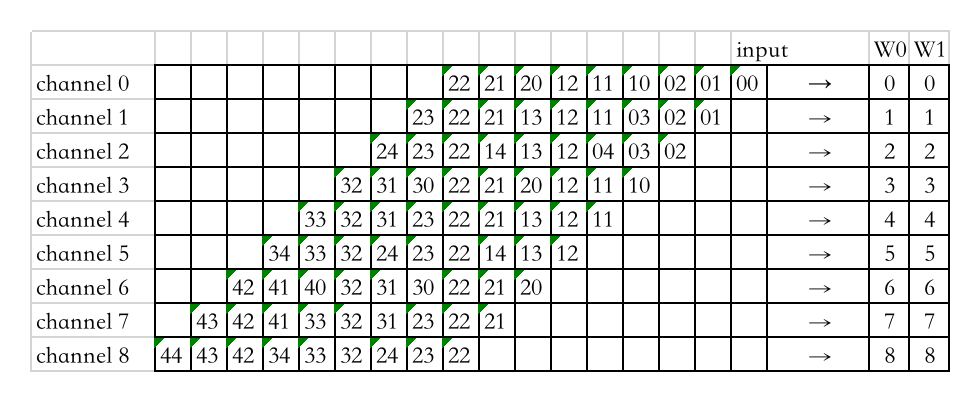
\includegraphics[width=15cm,height=7cm]{figures/input_systolic_array.png}
    \caption{数据输入脉动阵列示意图}
    \label{fig:systolic_data}
\end{figure}

\paragraph{padding}
对于边框填充,如果直接对输入数据进行修改,将会需要很大的存储来缓存数据,并且不排除会有很多读写的操作影响整个运算的效率。
因此,这里设计了一个专门用于填充边框的模块。
让它在把数据送入脉动阵列的通道以前,加入对应的填充值。
在把数据送入脉动阵列时,需要将数据按照执行卷积运算时的顺序依次送入脉动阵列。



\paragraph{图像数据的输入}
图像数据的输入模块具有一块缓冲来保存部分帧的图像数据。
控制图像数据输入模块的寄存器配置了特征图的尺寸和通道数。
同时,还配置了当前特征图属于哪一层的输入。
% TODO 将草稿纸上的状态机画上


\paragraph{权重的输入}
在本章中,已经提出了采用多路缓冲的思想来实现权重的输入方法。
控制权重输入的寄存器中,设置一个载入权重触发器,一个输入权重触发器,用来控制权重的载入和输出到脉动阵列。
控制寄存器中,设置权重尺寸、权重数量和所在层id,供固件作为参数输入。
% TODO 这里加上状态机的图示(已在纸上)


\subsubsection{脉动阵列}
% TODO 这里描述脉动阵列中运算单元的行为。
脉动阵列模块主要有3个部件组成:由运算单元组成的网络、权重缓冲区、输入管道、控制器。

% \begin{table}[!hpt]
%     \bicaption[PE的寄存器表]{PE的寄存器表}{Register Table Of PE}
%     \label{tab:firstone}
%     \centering
%     \begin{tabular}{@{}lllr@{}} \toprule
%         Type & Name & Description & Size \\ \midrule
%         input  & CLK  & 输入PE模块的时钟信号 & 32b \\
%         input  & RST  & 模块重置寄存器 & 16b \\
%         input   & SCLR   & 同步清零寄存器 & 16b \\
%         input   & A   & 输入参数A & 8b \\
%         input   & B   & 输入参数B & 8b \\
%         output   & Next\_A   & 输出到下一个PE的A & 8b \\
%         output   & Next\_B   & 输出到下一个PE的B & 8b \\
%         output & P & PE的运算结果P & 16b \\ \bottomrule
%     \end{tabular}
%   \end{table}

  
脉动阵列的设计和C模型实现,可以分为两个部分:脉动阵列模块的顶层设计和处理单元的设计。
处理单元(PE)的寄存器:时钟、重置、同步清零、输入参数A、输入参数B、输出给下一级的A、输出给下一级的
B、输出P值。


\subsubsection{算数逻辑单元}
算术逻辑单元是用来运算脉动阵列无法处理的运算的。

\paragraph{批规一化}
% https://zhuanlan.zhihu.com/p/34879333
归一化(normalization)可以理解为让每个特征图都有均值为0,方差为1的分布。
而批归一化(batch normalization)是为了简化完整的归一化的训练。
完整的归一化训练的时间复杂度和空间复杂度都很高,因此它对内存的要求较大,且训练的时间很长。
模块的输入参数有:特征图、形状的缩放系数$\gamma$、形状的位移系数$\beta$、数值稳定性常数$eps$、均值、方差

下面将展开说明批归一化的具体运算逻辑。
\subparagraph{计算均值和方差}
在训练模型时,需要计算得出mini-batch $B$的均值和方差,并记录下来。
在推理时,需要使用训练所得的均值和方差。  
均值的计算公式:
$$ \mu_{B} = \frac{1}{m} \sum_{i=1}^{m}x_{i} $$  

方差的计算公式:
$$ \sigma_{B}^{2} = \frac{1}{m} \sum_{i=1}^{m}(x_{i} - \mu_{B})^2  $$

\subparagraph{归一化}
在训练时,对mini-batch中的每一个特征$x_i$进行归一化处理
归一化的公式:
$$
        \hat{x}_{i} = \frac{ x_{i} - \mu_{B} }{ \sqrt{\sigma_{B}^{2}+\epsilon}}
$$

\subparagraph{推理inference}
该模块在运行时,只会进行推理(inference)。
在推理时,模块会使用到训练好的模型中的均值和方差的无偏估计量来进行批归一化,也就是:
$$ E(x) = E_{B}(\mu_{B}) $$    

$$ Var(x) = \frac{m}{m-1}E_{B}(\sigma_{B}^{2})  $$    

输出的特征图可以表示为:
$$ y = \frac{\gamma x}{\sqrt{Var(x) + \epsilon}} + ( \beta - \frac{\gamma E(x)}{\sqrt{Var(x) + \epsilon}} )  $$

因此,可以通过下面的伪代码来表述模块的运算逻辑:
\begin{codeblock}[language=python]
    scale = gamma / np.sqrt(var + eps)
    out = x * scale + (beta - mean * scale)
\end{codeblock}
先根据输入的参数算出缩放系数。
再使用缩放系数和位移系数处理特征图。

\paragraph{下采样和直接映射}
在ResNet的Basic Block中,需要使用下采样或者直接映射后,才能输出特征图到下一层。

\paragraph{全连接}
全连接层的核心操作是矩阵的乘法。
它能够把神经网络提取到的特征空间映射到样本标记空间。
对于权重,相当于做了特征加权。
因此,在ResNet18的网络结构最后做了平均池化和全连接。


\paragraph{Relu函数}
ReLU()函数全称叫作“修正线性单元”。
ReLU()函数的坐标轴图如图\ref{fig:relu}所示。
\begin{figure}[htbp]
    \centering
    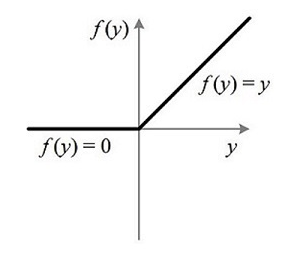
\includegraphics[width=12cm]{figures/ReLU.png}
    \caption{数据输入脉动阵列示意图}
    \label{fig:relu}
\end{figure}
它的公式如下所示:
$$
    f(x) = max(0,x)
$$


\paragraph{池化}
池化层通过对特征图中输入神经元的非重叠窗口(即池化窗口,每个窗口具有$K_x$×$K_y$个神经元)执行最大或平均运算,直接对输入特征图进行下采样。


%TODO 关于存储Multiple Bank的设计(状态机)
% 11/24 这一段需要重写,可能会搬到上面的某一段
% 本设计中,专门对存储进行了优化,区分开了不同的RAM区域来存储不用的数据,主要由以下几个区域:存储输入和输出数据的
% INRAM和OUTRAM、存储网络数据的NRAM、存储权重的WRAM、存储系统数据的SRAM以及存储临时数据的TRAM。拆分存储的设计
% 主要有以下两大好处:读写的带宽和避免冲突。
% 拆分存储之后,SRAM可以被调整为适当的读写宽度。假设输入和输出的宽度是$X_a \times K$字节,存储网络和权重数据的
% NRAM和WRAM为$X_a \times X_a \times K$字节。如果是用CPU或GPU,且未做优化的情况下,处理器只能按照固定宽度读取
% 数据。

